%! suppress = Quote


\section{Анализ предметной области}

В данной главе будет дан обзор системы типов языка Kotlin, на прикладных примерах будут описаны некоторые ограничения её выразительности и доступные решения.
После будет введено понятие Self-типа и показаны его преимущества как потенциального решения обозначенных проблем.
В завершение будут приведены приложения Self-типов в других задачах.

Для нашего изложения не принципиальна аккуратная формализация понятий объекта, наследования, подтипизации, полиморфизма с ограничениями и д.р.
Они будут даны прикладным образом как описание релевантных данной работе возможностей языка Kotlin.
Однако некоторые формализмы будут введены в главе~\ref{sec:theory} для демонстрации особенностей Self-типов, которые могут приводить к небезопасности системы типов (опр.~\ref{def:sound}).
В данной работе не ставится задачи формального доказательства безопасности, но встраивание в систему типов языка Kotlin новой возможности заведомо безопасным образом (в соответствии с существующими результатами, приведёнными в главе~\ref{sec:impls}), покрывая релевантные случаи использования, данные в разделе~\ref{subsec:applications}.


\subsection{Система типов языка Kotlin} \label{subsec:kotlin-typesystem}

\term{Kotlin} --- это объектно-ориентированный (ОО) промышленный язык программирования, поддерживающий компиляцию в Java bytecode, JavaScript и нативный код~\cite{jemerov2017kotlin}.

\begin{definition}
    \term{Система типов} --- это гибко управляемый синтаксический метод доказательства отсутствия в программе определенных видов поведения при помощи классификации выражений языка по разновидностям вычисляемых ими значений~\cite{pierce2002types}.
\end{definition}

\begin{definition}
    \label{def:subtype}
    Тип $B$ является \term{подтипом} типа $A$ ($A$ в таком случае~--- \term{надтип} $B$), если произвольное выражение типа $B$ может быть безопасно использовано в позиции, в которой ожидается выражение типа $A$~\cite{liskov1987keynote, pierce2002types}.
    Обозначение $B <: A$.
    Если два типа $C$ и $D$ не связаны отношением подтипизации, это обозначается так: $C \bcancel{<:>} D$.
    $C$ не подтип $D$: $C \bcancel{<:} D$.
\end{definition}

\begin{definition}
    \label{def:sound}
    \term{Безопасная (sound) система типов} --- всякая программа без приведений типов, в которой во время исполнения может возникнуть ошибка типизации, отвергается безопасной статической проверкой типов.
\end{definition}

Система типов языка программирования Kotlin обладает следующими основными свойствами~\cite{akhin2021kotlin}:
\begin{enumerate}
    \item Статическая --- проверка типов происходит на этапе компиляции;
    \item\label{itm:gradual} Gradually typed~\cite{siek2007gradual} --- система типов может накладывать более слабые ограничения, делегируя проверку типов времени исполнения программы для лучшей поддержки взаимодействия с кодом целевой платформы (реализуется в Kotlin с помощью \term{flexible types});
    \item Flow~\cite{pearce2013calculus} --- типизация значений в программе может зависеть от графа потока управления (реализуется в Kotlin через механизм \term{smart-casts}, см.~\ref{subsubsec:smart-casts});
    \item Null-безопасная --- вводится две вселенные типов: типы, которые содержат значение \mintinline{kotlin}|null|, \term{nullable} (обозначаются знаком вопроса в конце записи типа), и которые \mintinline{kotlin}|null| не содержат, \term{not-null};
    \item Без небезопасных неявных типовых конверсий;
    \item С поддержкой параметрического полиморфизма (опр.~\ref{def:param-poly}) с ограничениями (\ref{subsubsec:variance});
    \item С номинальной подтипизацией --- один тип является подтипом (опр.~\ref{def:subtype}) другого только в случае явного указания программиста в виде наследования (\ref{subsubsec:interitance-virtual}) или вариантности типовых параметров (\ref{subsubsec:variance});
    \item С общими верхним и нижним типами относительно отношения подтипизации --- тип \mintinline{kotlin}|Nothing| является подтипом любого типа, а \mintinline{kotlin}|Any?| --- супертипом любого типа;
    \item Безопасная (опр.~\ref{def:sound}), за исключением свойства~(\ref{itm:gradual}).
\end{enumerate}

\subsubsection{Наследование и виртуальный полиморфизм} \label{subsubsec:interitance-virtual}

Система типов языка Kotlin является \term{номинативной}.
Это значит, что отношение подтипизации нужно указывать явно и оно не следует из структуры значений типа.
Основным способом задания отношения подтипизации в Kotlin является \term{наследование}.

С помощью наследования же в Kotlin реализуется \term{виртуальный полиморфизм}.
Он заключается в том, что по ссылке базового типа происходит вызов метода наследника, если в действительность это ссылка на объект наследника.
\begin{minted}{kotlin}
    open class Base {
        fun method() { println("Base") }
    }

    class Derived : Base() {
        override fun method() { println("Derived") }
    }

    fun test() {
        val base: Base = Derived()
        base.method() // Печатает "Derived"
    }
\end{minted}

\subsubsection{Smart-casts}\label{subsubsec:smart-casts}

\begin{definition}
    \label{def:basic-block}
    \term{Базовый блок} --- непрерывная последовательность инструкций, всегда выполняющихся последовательно.
\end{definition}

\begin{definition}
    \label{def:cfg}
    \term{Граф потока управления программы (CFG --- control flow graph)} --- граф, составленный по программе из её базовых блоков.
    На рисунке~\ref{fig:cfg-example} приведён пример графа потока управления.
\end{definition}

\begin{figure}
    \centering
    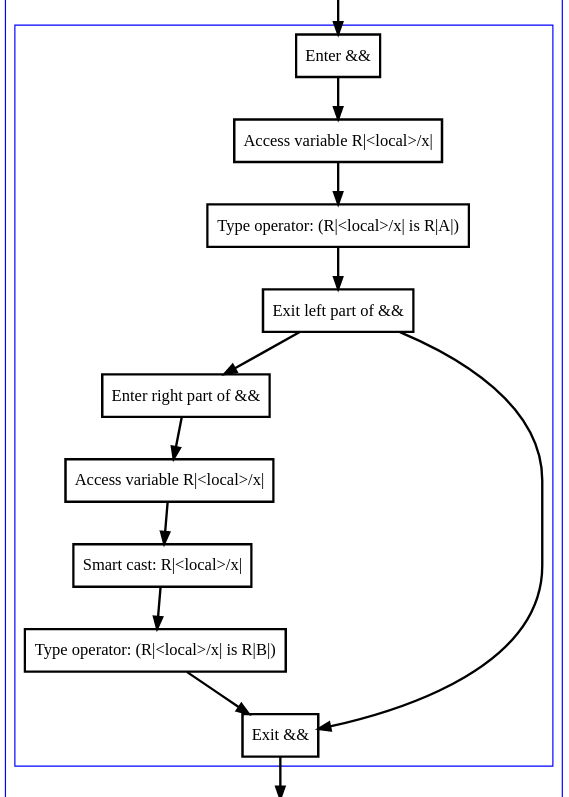
\includegraphics[width=0.8\linewidth]{fig/cfgExample}
    %! suppress = EscapeAmpersand
    \caption{Граф потока управления выражения \mintinline{kotlin}|x is A && x is B|.}
    \label{fig:cfg-example}
\end{figure}

\begin{definition}
    \label{def:intersection-types}
    \term{Тип-пересечение} --- тип, являющийся подтипом одновременно всех типов из пересечения.
    Обозначение для пересечения типов $A$, $B$ и $C$: $A~\&~B~\&~C$.
\end{definition}

Типы-пересечения являются примером типов, которые нельзя записать в Kotlin, то есть они не доступны программисту, но возникают в процессе вывода типов.
\begin{minted}{kotlin}
    interface A {
        fun aMethod() { /* ... */ }
    }

    interface B {
        fun bMethod() { /* ... */ }
    }

    class C : A, B
    class D : A, B

    fun test(cond: Boolean) {
        val intersection /* : A & B */ = if (b) C() else D()
        intersection.aMethod() // ok
        intersection.bMethod() // ok
    }
\end{minted}

\begin{definition}
    \label{def:start-cast}
    \term{Smart-casts} --- механизм уточнения типа за счёт информации, получаемой из графа потока управления программы.
\end{definition}

Например, если в условной конструкции проверяется принадлежность значения переменной типу, то в теле доступна информация о том, что тип этой переменной включает в себя тип из условия.
Это выражается с помощью типов-пересечений (опр.~\ref{def:intersection-types}).

\begin{minted}{kotlin}
    fun test(x: A) {
        if (x is B) {
            // x: A & B
            #\colorbox{green}{x}#.bMethod()
        }
    }
\end{minted}

\subsubsection{Параметрический полиморфизм и вариантность}\label{subsubsec:variance}

\begin{definition}
    \label{def:param-poly}
    \term{Параметрический полиморфизм} --- способность функции или класса работать с объектами различных типов путём абстрагирования реализации по \term{типовому параметру}.
    Тип, подставляемый вместо типового параметра~--- \term{типовой аргумент}.
\end{definition}

\begin{definition}
    \term{Параметрический полиморфизм с поддержкой ограничений}~--- параметрический полиморфизм, поддерживающий добавление ограничений на типы, которые можно использовать как типовые аргументы.
    В случае Kotlin, данным ограничением является требование на наличие у типа определённого супертипа.
\end{definition}

\begin{definition}
    \label{def:variance}
    \term{Вариантность} --- механизм языков с параметрическим полиморфизмом, позволяющий дополнять отношение подтипизации между параметризованными типами, когда типовые аргументы --- разные типы, связанные в свою очередь отношением подтипизации.
\end{definition}

В Kotlin вариантность может сообщаться типовому параметру класса как на стороне декларации, так и в месте использования этого класса.
В нашем изложении мы ограничимся только первым случаем, второй рассматривается аналогично.

\begin{definition}
    \label{def:type-positions}
    Возвращаемый тип функции будем называть типом в \term{исходящей позиции}.
    Тип параметра функции будем называть типом во \term{входящей позиции}.
    Тип, выступающий ковариантным типовым аргументом типа во входящей позиции, будем называть типом во \emph{входящей ковариантной позиции}.
    Аналогично для исходящей позиции и других вариантностей.
\end{definition}

\begin{definition}
    \label{def:type-position-sign}
    Типом в \term{положительной или ковариантной позиции} будем называть тип в исходящей позиции, исходящей ковариантной позиции или входящей контравариантной позиции\footnote{Определение типовых позиций даётся с практической точки зрения и не в самом общем случае, однако этого достаточно для данного изложения.}.
    Типом в \term{отрицательной или контравариантной позиции} будем называть тип во входящей позиции, во входящей ковариантной позиции и в исходящей контравариантной позиции.
\end{definition}

\begin{definition}
    \label{def:invariant}
    \term{Инвариантный типовой параметр} --- может использоваться в произвольных позициях деклараций методов класса.
    Не дополняет отношение подтипизации между параметризованными типами.
\end{definition}

\begin{minted}[escapeinside=??,mathescape]{kotlin}
    interface Inv<T> {
        fun id(x: ?\framebox{T}?): ?\framebox{T}?
    }

    // $\forall A, B\ldotp Inv\left<A\right> \bcancel{<:>} Inv\left<B\right>$
    fun test(b: Inv<B>) {
        // Отношение подтипизации не задано
        val a: Inv<A> = b // ошибка компиляции
    }
\end{minted}

\begin{definition}
    \label{def:covariant}
    \term{Ковариантный типовой параметр} --- может использоваться в положительных позициях деклараций методов класса.
    Параметризованный тип образует такое же отношение подтипизации, что и типовые аргументы.
\end{definition}

\begin{minted}[escapeinside=??, mathescape]{kotlin}
    interface Out<?\framebox{out}? T> {
        fun produce(): ?\framebox{T}?
    }

    // $B <: A \iff Out\left<B\right> <: Out\left<A\right>$
    fun test(b: Inv<B>) {
        val a: Inv<A> = b
    }
\end{minted}

\begin{definition}
    \label{def:contravariant}
    \term{Контравариантный типовой параметр}~--- может использоваться в отрицательных позициях деклараций методов класса.
    Параметризованный тип образует обратное отношение подтипизации относительно типовых аргументов.
\end{definition}

\begin{minted}[escapeinside=??, mathescape]{kotlin}
    interface In<?\framebox{in}? T> {
        fun consume(x: ?\framebox{T}?)
    }

    // $B <: A \iff In\left<A\right> <: In\left<B\right>$
    fun test(a: Inv<A>) {
        val b: Inv<B> = b
    }
\end{minted}

\subsubsection{Ресиверы в Kotlin}

\begin{definition}
    \label{def:receivers}
    Каждая функция, объявленная как метод или функция-расширение имеет специальные параметры (один или более), называемые \term{ресиверами}~\cite{akhin2021kotlin}.
    Такие параметры доступны как \mintinline{kotlin}|this| в теле функции.
\end{definition}

Далее в зависимости от контекста будем произвольно называть ресиверами такие специальные параметры, а так же объекты, используемые как соответствующие этим параметрам аргументы.
Например, в вызове \mintinline{kotlin}|"a".plus("b")| строка \mintinline{kotlin}|"a"| является объектом-ресивером для функции \mintinline{kotlin}|plus|.

Ресиверы в Kotlin могут быть трёх видов: dispatch, extension и context-ресиверы.

\begin{definition}
    \label{def:dispatch-receivers}
    \term{Dispatch-ресивер} --- ресивер, по которому происходит виртуальная диспетчеризация вызова.
\end{definition}

\begin{minted}[escapeinside=??]{kotlin}
    interface Base {
        fun greet()
    }

    class Derived : Base {
        override fun greet() {
            println("Hello")
        }
    }

    val b: Base = Derived();
    // b - dispatch-ресивер вызова
    b.greet() // Печатает "Hello"
\end{minted}

\begin{definition}
    \label{def:extension-receivers}
    \term{Extension-ресивер} --- ресивер, который является лишь специальным аргументом функции, но по которому не происходит виртуальной диспетчеризации вызова.
\end{definition}

\begin{minted}{kotlin}
    fun String.twice() = this + this
    // функционально аналогично определению
    // fun twice(String s) = s + s

    println("Y".twice()) // Печатает "YY"
\end{minted}

\begin{definition}
    \label{def:context-receivers}
    \term{Context-ресивер} --- ресивер, аналогичный extension-ресиверу (опр.~\ref{def:extension-receivers}), только для него не доступен синтаксис вызова функции явно через точку (не может быть явным).
\end{definition}

В дальнейшем изложении если не уточняется вид ресивера, имеется в виду dispatch или extension ресивер.

\subsubsection{Область видимости типа}

\begin{definition}
    \label{def:type-scope}
    \term{Область видимости типа}~--- множество функций, для которых объект данного типа может быть использован как ресивер.
\end{definition}

Например, функция \mintinline{kotlin}|plus| содержится в области видимости типа \mintinline{kotlin}|String|: \[(plus : String.(String) \to String) \in scope(String)\]


\subsection{Описание проблемы и возможных решений} \label{subsec:problem}

На данный момент система типов Kotlin недостаточно выразительна.
Так, в ней нет способа непосредственно сослаться на тип времени исполнения объекта-ресивера, на котором вызывается функция.
В то же время такая необходимость нередко возникает.
И при этом существующие решения, как правило, требуют либо существенного усложнения программных интерфейсов, либо написания большого объёма подверженного ошибкам рутинного кода, а также зачастую ограничивают возможности по обобщению и переиспользованию кода.
Многие из этих проблем решаются с помощью специальной поддержки в языке возможности записать тип времени исполнения ресивера функции.

В этом разделе мы рассмотрим некоторые наиболее распространённые случаи, на которых видна обозначенная нехватка выразительности системы типов Kotlin, а так же приведём возможные решения и укажем их недостатки.

\subsubsection{Шаблон <<Строитель>>}

Классическим примером, когда тип возвращаемой функции должен совпадать с типом ресивера, на котором она вызвана, является шаблон программирования <<Строитель>>.

Допустим, что у нас есть базовый класс для любого транспортного средства и строитель для него:

\begin{minted}{kotlin}
    open class Vehicle(val speed: Int)

    open class VehicleBuilder {
        protected lateinit var speed: Int

        #\framebox{open}# fun setSpeed(speed: Int): #\framebox{VehicleBuilder}# {
            this.speed = speed
            return this
        }

        open fun build() = Vehicle(speed)
    }
\end{minted}

Заведём наследника --- машину, имеющего своего строителя.
Чтобы переиспользовать функциональность строителя базового класса, унаследуем строителя наследника от него.
Однако возвращаемый тип метода \texttt{setSpeed}~--- всё ещё строитель базового класса, что не даёт возможность собирать объект машины в виде цепочки вызовов вида \mintinline{kotlin}|builder.setBase(1).setDerived(24)|.
Чтобы добиться такого синтаксиса, добавим переопределяющий метод с более специфичным возвращаемым типом и делегируем в нём вызов методу базового класса:

\begin{minted}{kotlin}
    class Car(speed: Int, val make: String) : Vehicle(speed)

    class CarBuilder : VehicleBuilder() {
        private lateinit var make: String

        #\framebox{override}# fun setSpeed(speed: Int): #\framebox{CarBuilder}# =
            super.setSpeed(speed) #\framebox{as CarBuilder}#

        fun setMake(make: String): CarBuilder {
            this.make = make
            return this
        }

        override fun build() = Car(speed, make)
    }

    fun testBuild(): Car = CarBuilder()
        .setSpeed(1)     // : #\framebox{CarBuilder}#
        .setMake("some") // : CarBuilder
        .build()
\end{minted}

Видим, что нам потребовалось написать ещё один метод с тривиальной реализацией и, более того, воспользоваться явным приведением типов.

Однако в Kotlin шаблон <<Строитель>> принято выражать с помощью анонимной функции с ресивером.
Так отпадает необходимость в записывании цепочек вызовов аналогичных приведённой выше.

\begin{minted}{kotlin}
    fun buildCar(block: CarBuilder.() -> Unit) =
        CarBuilder().apply { block() }.build()

    fun testBuild() = buildCar { x = 1; y = 2 }
\end{minted}

Тем не менее заметим, что для реализации второго подхода класс строителя должен быть изменяемым.

\subsubsection{Неизменяемые объекты}

Неизменяемые объекты играют значимую роль в современном программировании и являются основой распространённого функционального стиля программирования.
Важной задачей при написании кода является сокращение количества сущностей, которыми приходится единовременно оперировать, так как кратковременная память человека ограничена~\cite{lisman1995storage}.
Неизменяемость сущностей же позволяет не отслеживать постоянно их состояние (которое по определению не может измениться).
Так, для получения каждой модификации необходимо создавать новый объект.
Возможность же программировать таким образом обеспечивает развитие современных компьютеров и техник сборки мусора~\cite{jones2016garbage}.

Поэтому использование неизменяемых объектов считается хорошей практикой, а значит, язык должен предоставлять достаточное количество инструментов для простого и безопасного программирования с их использованием.
Однако при выстраивании иерархии неизменяемых объектов проблематичным оказывается использование метода базового класса, возвращающего объект ресивера или его копию:

\begin{minted}{kotlin}
    sealed interface Data {
        data class One(val a: Int) : Data
        data class Two(val a: Int, val b: Int) : Data

        fun update(a: Int): Data = when (this) {
            is One -> One(a)
            is Two -> Two(a, b)
        }
    }

    fun test() {
        val a = Data.Two(1, 2)
        val b: Data.Two = a.update(a = 2) // : Data, ошибка
    }
\end{minted}

Как мы увидим далее (см.~\ref{subsubsec:persistent}), на данный момент в Kotlin не существует простых и удобных способов добиться корректности типизации приведённого кода.

Такими объектами могут быть как простые неизменяемые структуры данных, так и, например, парсер-комбинаторы~\cite{hutton1996monadic}, содержащие в иерархии наследования различные методы порождения более сложных парсеров через комбинирование базовых друг с другом.

\subsubsection{Персистентные коллекции} \label{subsubsec:persistent}

Важным частным случаем неизменяемых объектов являются персистентные коллекции, которые на каждую модификацию возвращают новую ссылку на модифицированную коллекцию, в то время как коллекция, доступная по старой ссылке, остаётся неизменной~\cite{okasaki1999purely}.
Рассмотрим различные потенциальные способы задания интерфейсов библиотеки персистентных коллекций, используя существующие возможности языка Kotlin, а так же укажем недостатки этих подходов.

\paragraph{Типовые параметры с рекурсивными ограничениями} \label{par:recursive-generics}

Во-первых, требуемого можно добиться с помощью ковариантных типовых параметров с рекурсивными ограничениями.
Так, метод \texttt{add} должен вернуть новую коллекцию того же типа, но с добавленным элементом.
Обозначим это так, что \texttt{add} возвращает типовой параметр, представляющий собой конкретного наследника этого интерфейса, на котором вызывается метод.

\begin{minted}[escapeinside=??]{kotlin}
    interface PCollection<out E, ?\framebox{out S : PCollection<E, S>}?> {
        fun add(value: @UnsafeVariance E): ?\framebox{S}?
    }

    interface PList<out E, ?\framebox{out S : PList<E, S>}?> : PCollection<E, ?\framebox{S}?> {
        fun listSpecific()
    }

    class PListImpl<out E> : PList<E, ?\framebox{PListImpl<E>}?> {
        /* ... */
    }

    fun <T, ?\framebox{L}?> test(xs: ?\framebox{L}?, x: T) where ?\framebox{L : PList<T, L>}? {
        xs.add(x) /* : ?\framebox{L}? */ .listSpecific()
    }
\end{minted}

У данного подхода можно выделить следующие основные недостатки:
\begin{itemize}
    \item Паттерн рекурсивного ограничения распространяется по всему коду.
    \item В случае определения метода в любом месте иерархии, кроме финального класса, требуется явное приведение типов: \mintinline[escapeinside=??]{kotlin}|this as S|.
    \item Типовой параметр \texttt{S} может быть только однажды фиксирован в иерархии и более не может быть уточнён в наследниках.
    \item Такой подход является нетривиальным для понимания, особенно начинающими разработчиками.
\end{itemize}

\paragraph{Abstract override методы} \label{par:abstract-override}

Альтернативой может быть использование \term{abstract override методов}.
Теперь дополнительный типовой параметр не требуется, однако в каждом наследнике нужно добавить переопределяющий метод с более специфичным возвращаемым типом.

\begin{minted}[escapeinside=??]{kotlin}
    interface PCollection<out E> {
        fun add(value: @UnsafeVariance E): ?\framebox{PCollection<E>}?
    }

    interface PList<out E> : PCollection<E> {
        abstract override fun add(value: @UnsafeVariance E): ?\framebox{PList<E>}?
        fun listSpecific()
    }

    class PListImpl<out E> : PList<E> {
        /* ... */
    }

    fun <T> test(xs: PList<T>, x: T) {
        xs.add(x) /* : ?\framebox{PList<T>}? */ .listSpecific()
    }
\end{minted}

Видим, что теперь паттерн рекурсивного ограничения исчез, однако добавилась вспомогательная декларация.
У такого подхода можно выделить следующие недостатки:

\begin{itemize}
    \item Существенное количество рутинного кода: подобные декларации с более специфичными возвращаемыми типами требуется написать в теле каждого наследника.
    \item Нет контроля со стороны компилятора, что программист не забыл добавить подобные декларации во всех наследников при добавлении нового метода в базовый класс, что особенно чувствительно для разработчиков библиотек.
    \item Этот подход имеет место только для возвращаемых типов, типы параметров методов же должны совпадать по правилу переопределения функций базовых классов.
\end{itemize}

Несмотря на обширный список недостатков, подход с abstract override методами используется, например, в библиотеке персистентных коллекций языка Kotlin \texttt{kotlinx.collection.immutable}\footnote{\url{https://github.com/Kotlin/kotlinx.collections.immutable}}.

\paragraph{Ассоциированные типы}

\begin{definition}
    \label{def:assoc}
    \term{Ассоциированные типы}~\cite{chakravarty2005associated} --- это возможность объявить в базовом классе тип, определение которого будет дано только в реализации.
\end{definition}

Ассоциированные типы присутствуют в большом количестве языков без наследования, реализующих специальный полиморфизм через классы типов или трейты, например, Haskell и Rust.
Однако среди языков с наследованием ассоциированные типы встречаются не часто, например, в Swift и Scala.

Рассмотрим пример использования ассоциированных типов для интерфейсов персистентных коллекций на языке Scala, где ассоциированные типы носят название \term{abstract type members}\footnote{\url{https://docs.scala-lang.org/tour/abstract-type-members.html}}.

\begin{minted}{scala}
    trait PCollection[T] {
      #\framebox{type S}#
      def add(x: T): #\framebox{S}#
    }

    trait PList[T] extends PCollection[T] {
      #\framebox{type S <: PList[T]}#
      def listSpecific: Unit
    }

    class PListImpl[T] extends PList[T] {
      #\framebox{type S = PListImpl[T]}#
      override def add(x: T): #\framebox{PListImpl[T]}# = // ...
      override def listSpecific: Unit = // ...
    }
\end{minted}

Обозначим основные недостатки данного подхода:

\begin{itemize}
    \item Заметим, что аналогично подходу с abstract override методами в каждом абстрактном наследнике требуется уточнить ассоциированный тип.
    \item Также нет контроля со стороны компилятора, что это утонение не было забыто.
    \item Определение ассоциированного типа должно быть дано либо в абстрактном классе, либо в первом не абстрактном классе в иерархии.
    Дальнейшее уточнение ассоциированного типа ниже по иерархии наследования невозможно.
    \item В реализациях методов, находящихся выше по иерархии наследования, чем определение ассоциированного типа, требуется явное приведение типов.
\end{itemize}

Более того, реализация ассоциированных типов является очень нетривиальной задачей, если позволять вызывать методы, содержащие в сигнатуре ассоциированный тип, на экзистенциальном типе (см.~\ref{subsec:existentials}), так как нельзя полагаться, что тип, ассоциированный с одним значением, равен типу, ассоциированному с другим.
Поэтому приходится отслеживать, откуда пришло значение ассоциированного типа, и вместо установления подтипизации между двумя типами, сравнивать пути получения значений (значение может глубоко вложено как поле в композиции объектов).
Как правило, языки запрещают использовать такие методы на объектах экзистенциальных типов (Swift, Rust), а это почти все типы в ОО языках, что существенно снижает выразительность данного подхода.

Также стоит отметить, что на момент написания данной работы запроса от пользователей на добавление ассоциированных типов в Kotlin нет.


\subsection{Self-типы} \label{subsec:self-types}

Как мы увидели выше, на данный момент в Kotlin не существует удобного способа сослаться на тип времени исполнения объекта-ресивера.
Тем не менее у этой проблемы существует каноническое решение~--- Self-типы.

\begin{definition}
    \label{def:self-type}
    \term{Self-тип} --- тип ресивера (опр.~\ref{def:receivers}), на котором вызывается функция (тип \mintinline{kotlin}|this|'а).
\end{definition}

Self-типы встречаются так же как \term{рекурсивные типы} и \term{This-типы}~\cite{ryu2016thistype}.
А под названием Self-типы может подразумеваться нечто совершенно другое, как, например, в языке Scala\footnote{\url{https://docs.scala-lang.org/tour/self-types.html}}.

Пусть у нас есть базовый класс, в котором объявлен метод с \texttt{Self} в качестве возвращаемого типа.
Тогда при вызове этого метода базового класса на объекте наследника, мы сможем воспользоваться результатом как объектом типа наследника.
Вернёмся к примеру интерфейсов библиотеки персистентных коллекций (стр.~\pageref{par:recursive-generics} и~\pageref{par:abstract-override}).
Легко видеть, что вариант с Self-типами лишен перечисленных ранее недостатков.

\begin{minted}[escapeinside=??]{kotlin}
interface PCollection<out E> {
    fun add(value: @UnsafeVariance E): ?\framebox{Self}?
}

interface PList<out E> : PCollection<E> {
    fun listSpecific()
}

class PListImpl<out E> : PList<E> {
    /* ... */
}

fun <T> test(xs: PList<T>, x: T) {
    xs.add(x) /* : ?\framebox{PList<T>}? */ .listSpecific()
}
\end{minted}

Как было показано выше, Self-типы могут быть эмулированы с помощью дополнительных явных приведений типов и существенного количества рутинного кода.
Отсутствие поддержки Self-типов в языке и сложность их эмуляции может в некоторых случаях заставлять принимать менее удачные решения при разработке, выбирая подходы, не требующие Self-типов.
Таким образом, учитывая многочисленные запросы сообщества\footnote{\url{https://discuss.kotlinlang.org/t/self-types/371}}\footnote{\url{https://discuss.kotlinlang.org/t/this-type/1421}} и предоставляемое Self-типами удобство во многих ситуациях, было решено провести эксперимент по введению Self-типов в типовую систему языка Kotlin.


\subsection{Приложения Self-типов}\label{subsec:applications}

Self-типы могут быть полезны для реализации ещё нескольких популярных подходов и шаблонов программирования.
Перечислим некоторые из них в этом разделе.

\subsubsection{Рекурсивные структуры данных}

Self-типы нужны и для реализации рекурсивных структур данных, узлы которых могут состоять в иерархии наследования.
Допустим, что у нас есть класс, представляющий вершину дерева, и у него есть наследник, представляющий вершину с дополнительной функциональностью.
В таком случае Self-типы могут контролировать гомогенность типов вершин, а также позволяют вызывать методы наследника на результатах методов базового класса.

\begin{minted}{kotlin}
    abstract class Node<out T>(
        val value: T, val children: List<#\framebox{Self}#>
    )

    class BetterNode<out T>(
        value: T, children: List<#\framebox{Self}#> = emptyList()
    ) : Node<T>(value, children) {
        fun betterSpecific() = println(value)
    }

    fun test() {
        val betterTree = BetterNode(value = 2, children =
            listOf<#\framebox{BetterNode<Int>}#>(
                BetterNode(1, listOf(BetterNode(0))),
                BetterNode(4, listOf(BetterNode(3), BetterNode(5)))))
        betterTree.children
            .flatMap { it.children }
            .forEach { it.betterSpecific() } // Печатает "0 3 5"
    }
\end{minted}

\subsubsection{Шаблон <<Абстрактная фабрика>>}

В случае если требуется типизированным образом получать по элементу, созданному с помощью фабрики, её саму, Self-типы оказываются полезны в исходящей ковариантной позиции.

\begin{minted}{kotlin}
    abstract class Element<out F : Factory>(val factory: F)

    interface Factory {
        fun create(): Element<#\framebox{Self}#>
    }

    abstract class SpecificFactory : Factory {
        abstract fun doSpecific()
    }

    fun <F : SpecificFactory> test(element: Element<F>) {
        entity.factory.doSpecific()
    }
\end{minted}

\subsubsection{Шаблон <<Наблюдатель>>} \label{subsubsec:observer}

С помощью Self-типов можно абстрагировать логику хранения и оповещения наблюдателей.
В этом примере Self-тип используется во входящей контравариантной, то есть в положительной (ковариантной), позиции (опр.~\ref{def:type-positions}).

\begin{minted}{kotlin}
    abstract class AbstractObservable {
        private val observers = mutableListOf<(Self) -> Unit>()

        fun observe(observer: (#\framebox{Self}#) -> Unit) {
            observers += observer
        }

        private fun notifyObservers() {
            observers.forEach { observer ->
                observer(#\framebox{this}#)
            }
        }
    }

    class Entity : AbstractObservable {
        var color: Color = Color.Purple
            set(new: Color) {
                field = new
                notifyObservers()
            }
    }

    fun observer(entity: #\framebox{Entity}#) {
        println("New: ${it.color}")
    }

    fun test() {
        val entity = Entity()
        entity.observe(::observer)
        entity.color = Color.Blue // Печатает "New: Color.Blue"
    }
\end{minted}

\subsubsection{Алгебры} \label{subsubsec:algebras}

Ещё одним классическим применением Self-типов является кодирование алгебраических структур.
Так, интерфейс полугруппы мог бы выглядеть следующим образом.

\begin{minted}{kotlin}
    interface Semigroup {
        infix fun add(other: Self): Self
    }
\end{minted}

Однако уже, например, моноид с одним константным символом таким образом уже задать не получится, так как любой метод всегда принимает как минимум один аргумент (\mintinline{kotlin}|this|).
Более того, как мы увидели выше в~\ref{subsec:self-types}, использовать Self-типы во входящей позиции небезопасно.

В современном Kotlin существует другой механизм, который больше подходит для описания алгебр,~--- контекстные ресиверы (опр.~\ref{def:context-receivers}).

\begin{minted}{kotlin}
    interface Semigroup<S> {
        infix fun S.add(other: S): S
    }

    interface Monoid<M> : Semigroup<M> {
        val empty: M
    }

    object StringMonoid : Monoid<String> {
        override val empty: String = ""
        override fun String.add(other: String): String = this + other
    }

    context(Monoid<T>)
    fun <T> concat(vararg xs: T): T =
        xs.fold(empty) { acc, x -> acc add a }

    fun test() {
        with(StringMonoid) {
            println(concat("a", "bc", "d")) // Печатает "abcd"
        }
    }
\end{minted}


\newpage


\subsection{Цель и задачи работы}

Таким образом, можем сформулировать цель и задачи данной работы.

\textbf{Цель: } Разработать дизайн Self-типов для языка Kotlin на основании опыта других языков и реализовать поддержку Self-типов в компиляторе kotlinc.

\textbf{Задачи:}
\begin{enumerate}
    \item Выделить особенности существующих решений: возможные значения Self-типа, допустимые позиции Self-типа и меры по обеспечению безопасности системы типов;
    \item Интегрировать Self-типы в типовую систему языка Kotlin на основании проведённого анализа решений;
    \item Реализовать поддержку Self-типов в компиляторе kotlinc.
\end{enumerate}
